\subsection{Basic Attribute-Based Encryption}
In the following sections we will habe a look at the different attribute based encryption schems. We will extract characterisitics of thouse schemes to cluster them, select a repectable candidate from each of those schemes and to finally, make a practical performance anaylsis of thouse schemes. 

A suitable candidate in the field of attribute based encryption scheme is a scheme that satisfies the requirements stated in section \ref{sec:requirements}. The requirements are a super set of thouse defined in \cite{lee2013survey}. For the basic \ac{ABE} schemes we will focus on the requirements \req{C1}, \req{C3}, \req{C5} - \req{C8} and optional requirements \req{O1} and \req{O2}.
The general requirements \req{B1} and \req{B2} will be evaluated by pratical a performance and scalability anaylsis.

\subsubsection{Collusion resistance (C2 requirement)}
Lets construct a very basic attribute based encryption scheme to clarify the importance of collusion resistance. Assume baisc \ac{RSA} cryptography. We setup an \ac{AA} which combines attributes to \ac{RSA} public-private key pairs. Attribute "student" gets bound to $K_{PR(s)}$ for the private key and $K_{PU(s)}$ for the public key. Attribute "works at TU Berlin" gets bound to the Key $K_{PK_PR(tu)}$ and $K_{PU(tu)}$ respectivly. Now, we setup our very own first ABE scheme. The AA can pin the public keys of each attributes to its public billboard so that every entity in the system can encrypt for thouse attributes. Each user who is currently a student receives a copy of the private key $K_{PR(s)}$ and each user who is currently working at TU Berlin receives a copy of $K_{PR(tu)}$. 

A user, lets call her for historical reason Alice, wants to share content with all students that are also working at TU berlin. She encrypts the plaintext $p$ with both public attribute keys $c = K_{PU(s)}(K_{PU(TU)}(P))$ and publishes the ciphertext $c$ to a public CSP so that everyone can download it. Students that are working at TU Berlin owning both private keys can decipher the ciphertext by applying both private keys in reverse order $K_{PR(TU)(K_{PR{s}}(c)}$.

The attentive reader will have notice a cural security leak in this scheme. This \ac{ABE} scheme is not cullusion restiant. In fact, collusion restistance is a core requirement of any attribute-based encryption schemem. On paper it is defined as the impossibility of any two attribute holder to combine their attributes to archive a higher level of encryption. Lets assume that Bob is a student and Eve is working at \ac{TU} Berlin. Both users received their private key. Now they can simply exchange their attribute keys so that they are both able to decipher the ciphertext even if they severativly don't own both attributes.  

Usally collusion restance is ensured by issuing each user a private key that is blinded by a random value. This random value will vanish on decryption. However, if two users collude they will mix their blinded values resulting a plaintext that is still by some unknown value. 

\subsubsection{Bilinear Mappings}
To ensure collusion resistance bilinnear maps are comonly used. They are a tool for \textit{cytrographic pairings} and define the relationship between cyclic groups of the same (prime) order. A cyclic group $G$ is defined by an generator $g$ of that form that each $g^n \in G$ with $n \in \mathbb{Z}$ complelty desribes each element in the group $G$.

A bilinear map function $e$ is now defined as the mapping between two groups of the same order $G_1$ and $G_2$ into $G_t$:

$$ e : G_1 \times G_2 \rightarrow G_t $$
$$\text{ such that for all } g_1 \in G_1, g_2 \in G_2, a, b \in \mathbb{Z}$$
$$e(g_1^a, g_2^b) = e(g_1, g_2)^{ab}$$

%In some schemes $G_1$ and $G_2$ relate to the same cyclic group. Another nice fact is that the \textit{Decisional Bilinear Diffie-Hellman Problem} becomes easy computable. 

This contruct of pairings is used by many schmes to either distribute a secret or computing the secret without ever revealing it. To now ensure collusion resistance with this technique normally a user specific id (\ac{UID}) is generated and bound to the exponent of the user's attribute private key. The decryption method will be designed in that way that the blinding of the attribute private key will vanaish.   

\subsubsection{\ac{KP-ABE}}
In Key-Policy Attribute-Based Encryption (\ac{KP-ABE}) \cite{goyal2006attribute}, is a \ac{ABE} technique that assoizates chiphertexts with attributes that fullfill the policy embedded in the key addressed to a user. 

To evaluate if a policy matches given attributes an \textit{Access Tree} or \textit{Linear Secrect Sharing Matrix} (\ac{LSSS}) is used. While both representations represent the same boolean formular a \ac{LSSS} is often more efficient. For a better explanation the model of an access tree will be used. For each node of this tree it is evaluated whether the children satisfy a certain condition. This might be implemented as \textit{OR} or \textit{AND} treshhold gates. While \textit{OR} can be expressed as $1$-out-of-$n$ children need to satisfy the condition, \textit{AND} conditions are $n$-out-of-$n$ threshhold gates meaning all children need to satisfy the condition. This approach is a monotonic access strcture and often refered as \textit{Threshhold Security} or \textit{Treshhold Access Strcutre}. 

The initial paper did leck some basic requirements that was improved by other work. Such as a fix-length cipher text, attribute revocation. Further, the authors stated that users, onces issued a policy, are able to delegate a subset of their access tree to other users. Users themself could act as a new attriubte authority to issue other uses a subset of thier access policy. While this is a nice feature for some use cases, in a cloud system the company would like to restrict this delegation or would like to be able to track traidors selling their private keys as a blackbox decryption.

This encryption scheme was ment as a broadcasting encryption scheme. Used by radio providers so that they can address any user that bought a paid membership to distribute premium content. However, since the policy was bound to the users key it is not possbile to address a ciphertext to a specific user group without knowing who exaclty persesses the right policy. Only the central authority, which issued the users privayt keys in the first place, would know who could decipher the encrypted text. This fact renders \ac{KP-ABE} impractical for tha application in a cloud sharing scheme. User would simply don't know who are able to decrypter the cipher text. 

The certainly very specific use case of \ac{KP-ABE} probably led to the circumstances that not much paper using this technique exists. Even so that we could not find any paper satisfying all requirements previously specified. We found only paper that implemented direct revocation using negation of attributes \cite{lewko2010revocation}. This would in turn lead to the fact that users private key sizes would grow with each revoced attribute. 

\subsubsection{\ac{CP-ABE}}
On the other side there is Cipher-text policy Attribute-Based Encryption (\ac{CP-ABE}) \cite{bethencourt2007ciphertext}. \ac{CP-ABE} assigns ciphertexts with a policy and user keys with attributes. This enables \ac{CP-ABE} to be much more flexible and verbose in comparison to \ac{KP-ABE}. The big adventages was (similar to \ac{KP-ABE}) that the need for a central authentication server was obsulte. Each ciphertext could simple accessed by each user and only thouse who have the right attribute set present are able to decipher the ciphertext. 

The lack of revocation \req{C8} and the need for a large attribute and user universe was huge \req{C5}. Revocation means that a system manager could revoke attributes from users or even the user as such. In modern company settings an required feature to ensure forward secrecy. Large attribute universe on the other hand describes that the attributes that can be distributed by the \ac{AA} are somewhat so large that it is unlikly that a running system will run out of attributes to issue. 

The first proposal of a revocation scheme in \ac{CP-ABE} was in 2010 \cite{liang2010ciphertext}. This scheme used a similar approach like \ac{LKH} to make the revocation process effient. In 2016 Lui \textit{et. al} \cite{liu2016practical} proposed a recovable \ac{ABE} scheme that supported traidor tracing and large attribute universe. However, both scheme were restricted to a fix number of users or a limited attribute universe. Which rendered them pratical not applicable.  

\subsubsection{Non-monotonic access strcutre of \ac{ABE}}
While monotonic access structures can describe \textit{AND} or \textit{OR} gates, non-monotonic access structure can also refere to \textit{NOT} gates. This adds another layer of find-ganylarity into the system. While in monotonic access strctures user get an attribute assigned they have access to all topics addressed to this attribute. In non-monotonic strctures, first intoduced by Ostrovsky \textit{et. al.} \cite{Ostrovsky:2007:AEN:1315245.1315270}, certain topics may be excluded. 

Take for example Alice who wants is an intern in the Top Secret company. In monotinic access strcutre she would receive both attribute private keys from "Intern" and "working in Top Secret Company". Since than she would be able to decipher all content addressed to all employees at the Super Secret company. However, some content might be so confidential that interns shell not be able to access them. This exclusion would not be possible. With non-monotonic access structure an administrator may want to encrypt certain information with the policy "working in Top secret Company AND NOT intern".  

While being an imported field in the boolean formular and fine-grand access control domain, non-monotonic access structures did not gain the same attention as \ac{CP-ABE} or \ac{KP-ABE} did. As an candidate which shell represent this \ac{ABE} topic \cite{10.1007/978-3-642-54631-0_16} \ac{CP-ABE} implementation will be used. With negation of attributes revocation becomes more or less trivial. Each attribute can be versioned and simply exlcuded on encryption. While this approach is not scalable over time it is simple enough to be implemented in some schemes.   

\subsubsection{Multi-Authority Attribute Based Encryption}
Ontop of the previos mentioned schemes emerged a new sub topic of \ac{ABE}: \textit{Multi-Authority Attribute Based Encryption} (\ac{MA-ABE}). The main motivation was that a single \ac{AA} is not practically applicable. In the real world we face different domain each maintaining it own attributes. 

\ac{MA-ABE} while beeing a roughly young field of \ac{ABE} encryption technique enjoyed a lot of attention in the research area. In addition to the normal requirements like collusion resistance and revocation mechanism, \ac{MA-ABE} also deals with the question on how to deescalate the global decryption power of the central authority (\ac{CA}). 

A setup of a \ac{MA-ABE} system looks quite similar over the field of related work. On system inizialisation we setup the \ac{CA}. The purpose of the \ac{CA} is to bootrap new Attribute Authoritieis (\ac{AA}) which then will administer their domain. In this domain users and attributes of the \ac{AA} are located. After the \ac{CA} bootstraped all \ac{AA}s and all users are registed it could in theority go offline. 

To ensure system wide collusion resistance each user usally gets a unique user identifiery (\ac{UID}) assigned. This \ac{UID} is issued by the \ac{CA} which is the only entity having an overview about the whole system. 

A suitable condidate to compare \ac{MA-ABE} to the previous introduced schemes is \textit{hirachical attribute based encryption} (\ac{HABE}, section \ref{sec:HABE}). In short \ac{HABE} is structured around the idea of attribute administration delegation. The strcture can be imaged like the domain name system. On top level there is the root master administating the whole domain. He can delegate power in form of attribute issuing und user setup to sub entities. This sub entities can again forward a subset of their power to their childen. For a complete explenation see \ref{sec:HABE}. We will use \cite{Wang:2010:HAE:1866307.1866414} as representiv candidate for \ac{MA-ABE}. 

\subsubsection{Comparison}
To compare the selected representived of the previous section we choose the charm framework\footnote{\url{http://charm-crypto.io/}}. Here we can already find implementations for the sutable \ac{KP-ABE} candidate \cite{lewko2010revocation} and for non-monotonic \ac{CP-ABE} \cite{10.1007/978-3-642-54631-0_16}. The other two schemes such as \ac{CP-ABE} \cite{liu2016practical} and \cite{wang2011hierarchical} where implemented by us in a github frok of the charm repo\footnote{\url{https://github.com/Anroc/charm}}. 

\begin{table*}[!ht]
\centering
\begin{tabular}{l 					| l 				| l 						| l 				| l}
									& \textbf{LSW 08} \cite{lewko2010revocation}	& \textbf{YAHK 14} \cite{10.1007/978-3-642-54631-0_16} & \textbf{LW 14} \cite{liu2016practical} & \textbf{WLWG 11} \cite{Wang:2010:HAE:1866307.1866414} 	\\
\req{Scheme}						& \ac{KP-ABE}		& Non-Monotone \ac{CP-ABE} 	& \ac{CP-ABE} 		& Hirachical \ac{CP-ABE}		\\ 
\req{Security scheme}				& Biliniear maps 	& Binilnear maps 			& Biliniear maps 	& Biliniear maps 				\\
\req{Expression of access policy}	& \ac{LSSS}			& \ac{LSSS} matrix 			& \ac{LSSS} matrix 	& \ac{DNF} 						\\ 
\end{tabular}
\caption{Scheme description. }
\label{tab:comparison_baic_abe_overview}
\end{table*}
\begin{table*}[!ht]
\centering
\begin{tabular}{l 	| l					| l 				| l 				| l}
					& \textbf{LSW 08} \cite{lewko2010revocation}	& \textbf{YAHK 14} \cite{10.1007/978-3-642-54631-0_16} & \textbf{LW 14} \cite{liu2016practical} & \textbf{WLWG 11} \cite{Wang:2010:HAE:1866307.1866414} 	\\
\req{C1}			& Yes				& Yes 				& Yes 				& Yes 				\\
\req{C2}			& No				& No 				& No 				& Yes 				\\ 
\req{C3}			& No				& No 				& No 				& No 				\\ 
\req{C4}			& No				& No 				& No 				& No 				\\ 
\req{C5}			& Yes				& Yes 				& Yes 				& Yes 				\\ 
\req{C6}			& - 				& - 				& -					& Yes				\\
\req{C7}			& -					& - 				& - 				& No 				\\
\req{C8}			& Yes				& Yes				& Yes				& Yes				\\
\req{O1}			& No 				& No 				& Yes 				& No 				\\
\req{O2}			& Yes+ 				& Yes+				& Yes				& Yes-				\\
\end{tabular}
\caption{}
\label{tab:basic_abe_comparisons}
\end{table*}

In table \ref{tab:comparison_baic_abe_overview} the different scheme techniques are listed.  And in Table \ref{tab:basic_abe_comparisons} this schemes are compared to the requirements of section \ref{sec:requirements}. 

From table \ref{tab:basic_abe_comparisons} it is clear that no scheme fully fulfill all requirements. However, they reveal a good indicator where we should look next. WLWG 11 clearly makes the race here satisfying 6 of 10 of the requirements. 

\req{C6} and \req{C7} could not be sutisfied by LSW08, YAHK14 or LW14 since they are not designed to support multible authorities. 
\question{Should I respect \ac{MA-ABE} also here?}
Lets have a look at \req{O2}. LSW08 and YAHK14 both supports fine grant access controll by using a \ac{LSSS} access structure. Also both implement non-monotonic access structes which give them the extra plus. LW14, on the other hand, does not support negation of attributes, but support an arbirary access strcture like LSW08 and YAHK14. WLWG11, however, does only support access strcutures in \ac{DNF} form which makes this scheme somehow restriced in expressivness. 

\begin{figure*}[!ht]
\centering
    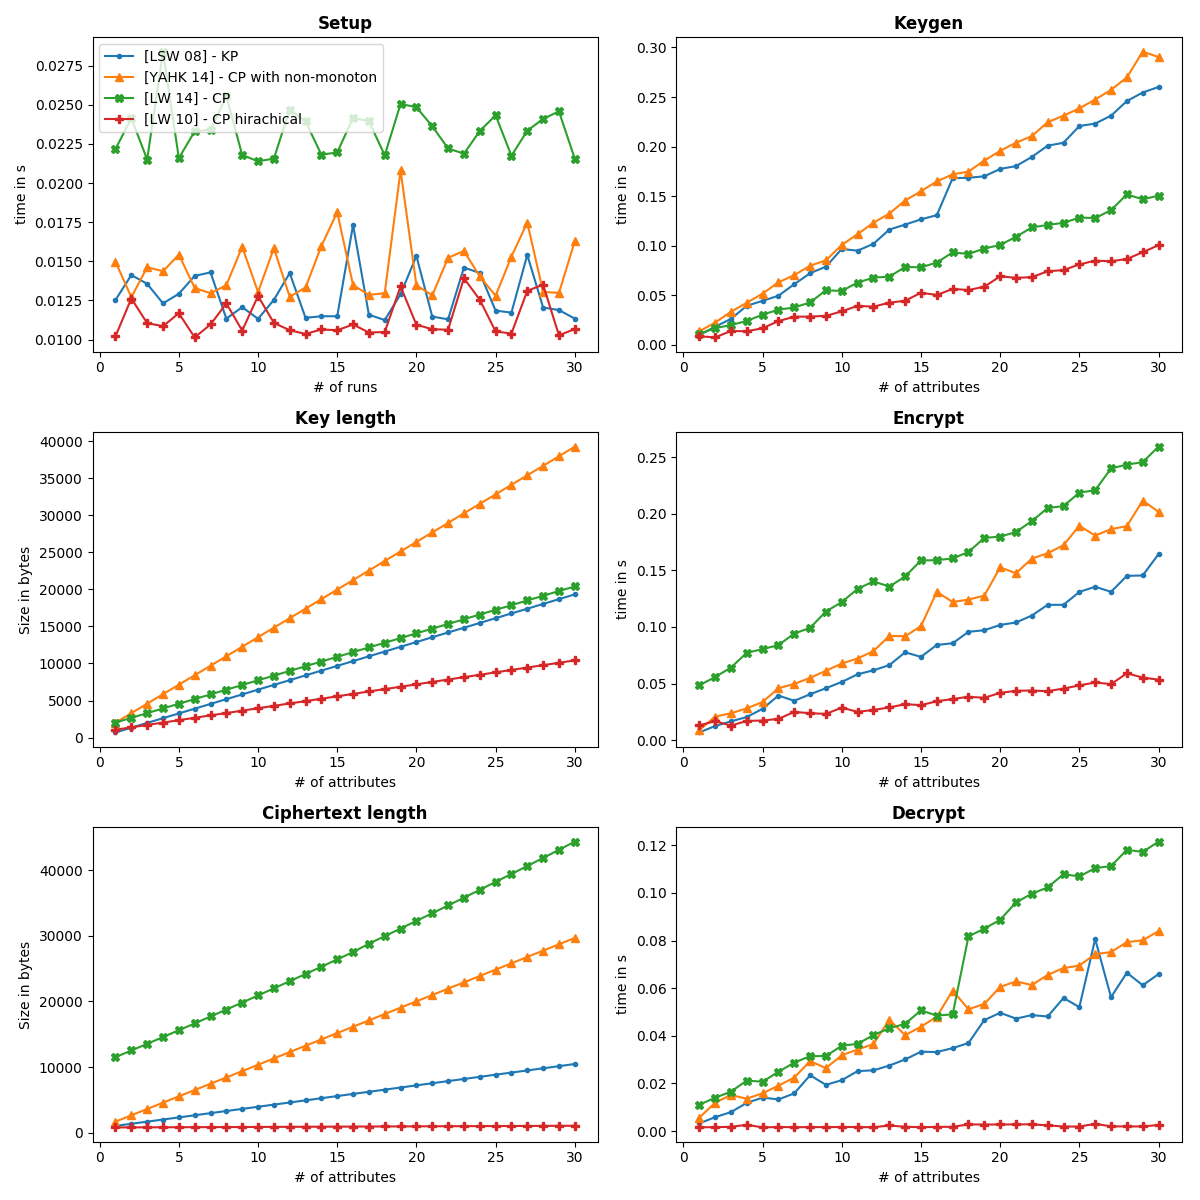
\includegraphics[width=1\linewidth]{img/basic_abe_comparisons.png}
    \caption{Performance and scalability comparison between the chosen schemes with increasing number of attributes. The policy for each new attribute $a_k$ with $a_k \in A$ was defined as $\bigwedge\limits_{a \in A}^a a$. Key generation relates to the creation of users key pairs given an accesspolicy or attribute set.}
    \label{fig:basic_abe_comparison}
\end{figure*}

Notable about the comparison in figure \ref{fig:basic_abe_comparison} is that while \ac{KP-ABE} (LSW08) was expected to have the biggest overhead in Keygeneration compared to the \ac{CP-ABE} schemes and the lowest in encyrption, since no policy has to be parsed and computed here. However, none of the both assumtions was true. It seams more like the time complexlity and runtime of the different algorithms suerly depends on the design of the scheme. 

Also remarkable is that WLWG11 has the best overall performance. But it must also be noticed that in the we did not include the attribute authoirity key generation. While the paper claimed to have an constant overhead on decryption it is impressive to see that it holds true. 

While the plaintext message remained contant it is clearly visible that the ciphertext length groth linearly with the number of attributes. 

Due the greate performance and the coverage of the most of the requirements of the hirachical attribute based encryption technique, the field of multi-authority attribute based encyrption will be evaluated in more depth. Regardless of the great scalability of the \ac{HABE} it comes with a non neglegtable disadventage. The root master and the top level domain master have both global decryption power. For each user regardless of the company affiliation the administator of the system will always be able to dechipher ciphertexts of thouse users. This would break end-to-end encryption complelty. So clearly we would favor solutions that support different attribute authorities so that each company can administer their own domain seperatly from each other, but we want also that root, while beeing able to boostrap new attribute authorities, is not able to decihper any ciphertext. 


